\documentclass{article}

\usepackage{txfonts}
%\usepackage{amssymb}
%\usepackage{fancyhdr}
\usepackage{ctex}
\let\iint\undefined
\let\iiint\undefined
\let\iiiint\undefined
\let\idotsint\undefined
%\renewcommand{\thefootnote}{\fnsymbol{footnote}}
\usepackage{xcolor}
\usepackage{amsmath}
\usepackage{mathrsfs}
\usepackage{float}
\usepackage{verbatim}
\usepackage{listings}
\newtheorem{lemma}{Lemma}
\newtheorem{theorem}{Theorem}
\newtheorem{definition}{Definition}
\newtheorem{corollary}{Corollary}
\usepackage{graphicx}
%\usepackage{authblk}
%\textheight=720pt
\usepackage[top=1in, bottom=1.1in, left=1.25in, right=1.25in]{geometry}
%\linespread{1.25}
%\phone{86-18701698932}
%\usepackage[scaled]{uarial}
%\usepackage[T1]{fontenc}
\usepackage[english]{babel}
\usepackage{booktabs}%for \toprule
\usepackage{float}
%\bibliographystyle{plain}
%\newcommand*{\MyPath}{../Notes}%
\graphicspath{{./Fig/}{fig/}}

\makeindex
\begin{document}
The following analysis is based on a sample corpora(english as source, chinese as target and align). I set both vocabulary sizes as 10000.
\begin{itemize}

\item[1. ] the first figure is about whether the unk in target sentence has aligned words in source sentence.  
\begin{figure}[H]
\centering
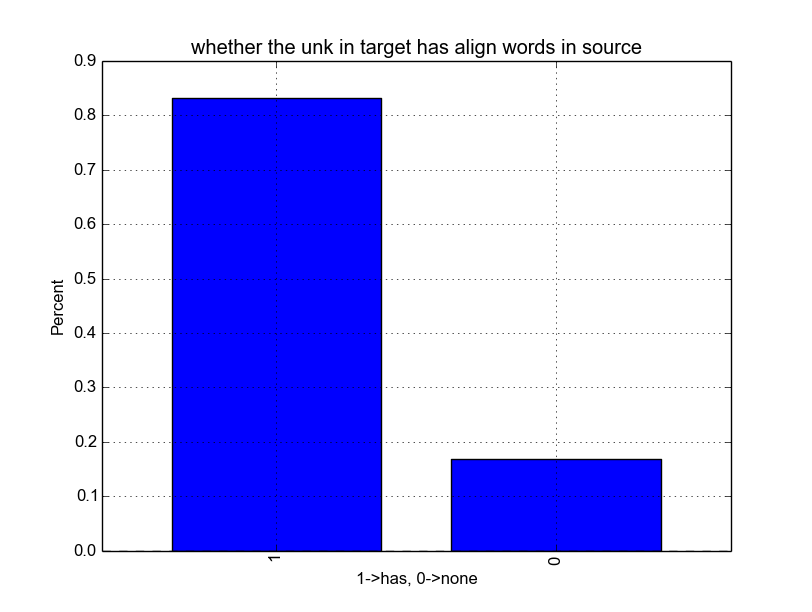
\includegraphics[height=8.5cm]{figure_6.png}
\caption{for over 80\% cases, the unk has aligned words in source sentence}
\end{figure}

\item[2. ] if the unk has aligned words in source sentence, how many words(unk or not) does the unk align to
\begin{figure}[H]
\centering
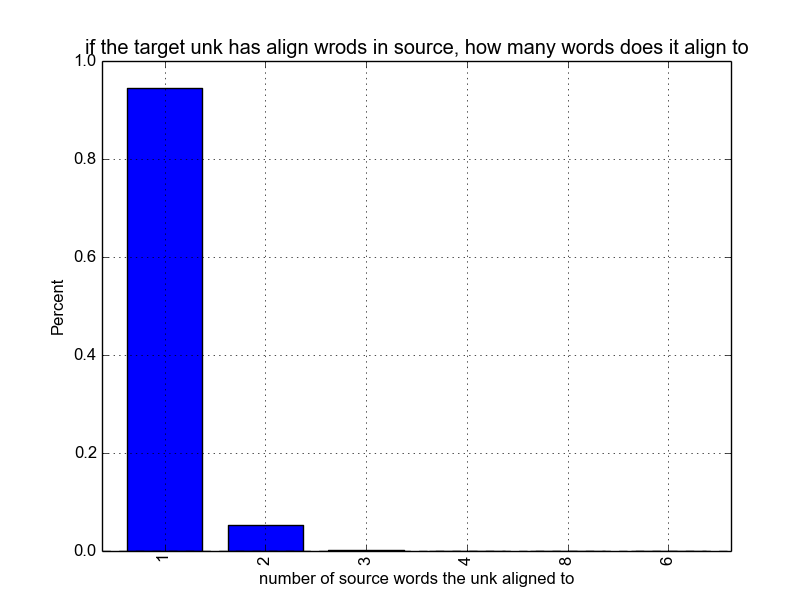
\includegraphics[height=8.5cm]{figure_1.png}
\caption{for over 90\%cases, a unk aligns to only one word in source sentence}
\end{figure}

\item[3. ] for those source words that aligned to the target unk, how many unk(source unk) do they contain  
\begin{figure}[H]
\centering
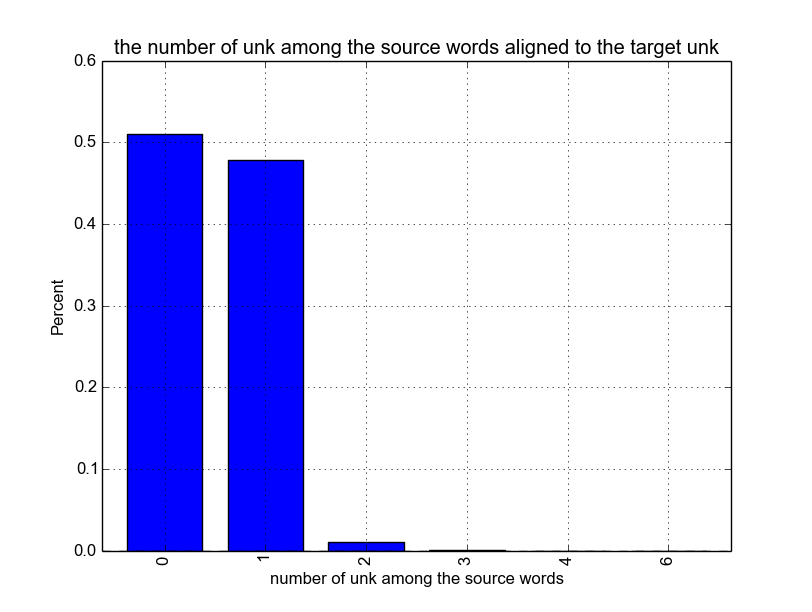
\includegraphics[height=8.5cm]{figure_2.png}
\caption{there is no unk in the aligned source words for almost 50\% cases and only one unk for another 50\% cases}
\end{figure}

\item[4. ] this figure measures the same thing by portion
\begin{figure}[H]
\centering
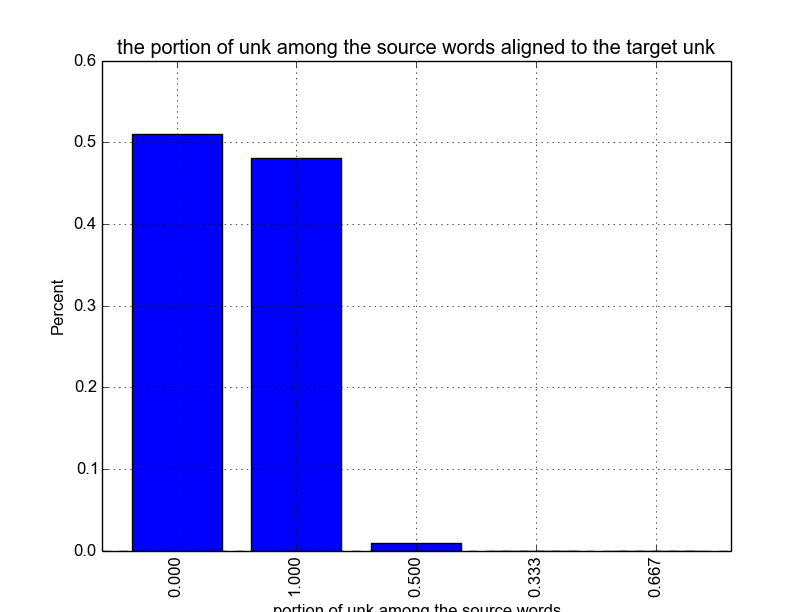
\includegraphics[height=8.5cm]{figure_3.png}
\caption{the result is the same as in the above figure}
\end{figure}

\newpage
\item[5. ] for those source words that aligned to the target unk, the relative distances between them and the target unk
\begin{figure}[H]
\centering
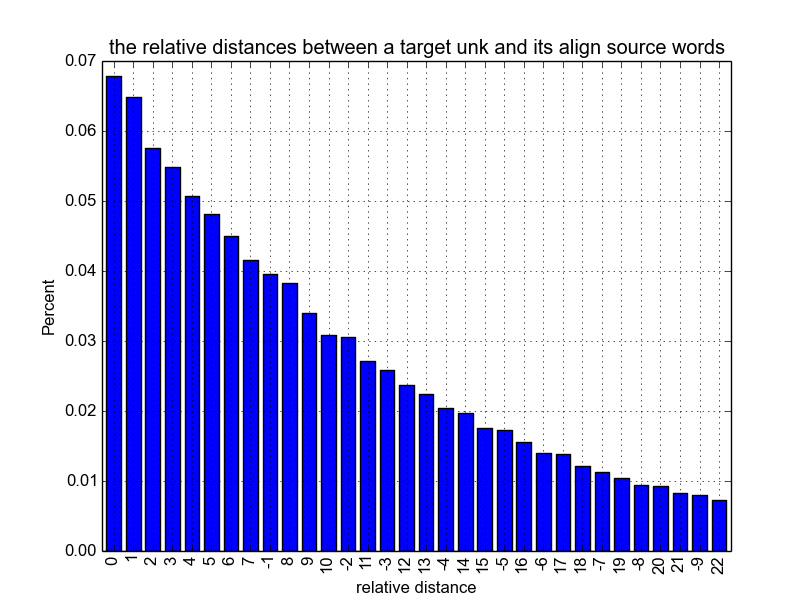
\includegraphics[height=13.0cm]{figure_4.png}
\caption{it looks like english word in a alignment pair is more likely to be on the right of chinese word  }
\end{figure}
\newpage
\item[6. ] for those source words that aligned to the target unk, the relative distances pattern between them and the target unk
\begin{figure}[H]
\centering
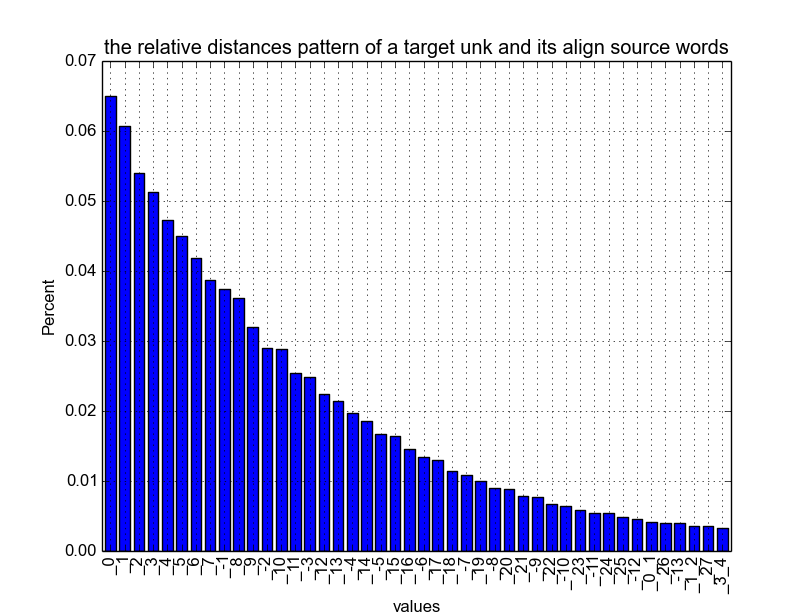
\includegraphics[height=13.0cm]{figure_5.png}
\label{fig:dicesetdoc_grammar}
\caption{the $'\_'$ in the labels of x-axis emans a aligned word and the number following $'\_'$ means the relative distance. Most of the time, there is only one aligned word for a target unk and the distances distribution between them looks close to the above figure.}
\end{figure}
\end{itemize}

\end{document}